%!TEX TS-program = pdflatex

%%%% Latex preamble and page formatting %%%%

\documentclass[12pt]{article}  % larger font to compensate for long lines with fullpage
\usepackage[utf8]{inputenc}
\usepackage[T1]{fontenc}
\usepackage[pdfborder={0 0 0}]{hyperref} % use hyperref without borders
\hypersetup{
    pdftitle = {Network Service Interface Topology Service},
    pdfauthor = {Jeroen van der Ham},
    pdfsubject = {Specification of the syntax and distribution mechanism of the topology service},
    pdfkeywords = {network topology distribution}
}
\usepackage{ifpdf}
\usepackage{ifthen}
\usepackage{graphicx}
\usepackage{url}
\usepackage{color}
\usepackage{listings}
\usepackage[title,titletoc]{appendix}
% Read pictures from img/ and current directory
\graphicspath{{img/}{./}}

%%% GWD/GFD header follows %%%
% Feel free to make changes, as long as your document follows the guidelines of GFP.152

\usepackage[numbers]{natbib} % Use [1] for references, 
\bibliographystyle{plainnat} % References show full author name(s) and document URL

\usepackage[sf,compact]{titlesec} % Use sans-serif for section headers

\usepackage[titles]{tocloft} % Format table of contents
% (tocloft is used, since titletoc is incompatible with xetex.)
\renewcommand{\cftsecfont}{\sffamily}
\renewcommand{\cftsubsecfont}{\sffamily}
\renewcommand{\cftsubsubsecfont}{\sffamily}
\renewcommand{\cftsecpagefont}{\sffamily}
\renewcommand{\cftsubsecpagefont}{\sffamily}
\renewcommand{\cftsubsubsecpagefont}{\sffamily}
\renewcommand{\cftsecleader}{\cftdotfill{\cftsubsecdotsep}} % dots for sections the same as for sections
\setlength{\cftbeforesecskip}{0.5ex}

\usepackage{parskip} % Blank lines between paragraphs, no indentation.

% font style for headers and footers
\newcommand{\headerstyle}{\sffamily} % sans-serif

% Set page margins
\usepackage{fancyhdr}
\addtolength{\headheight}{15pt}
\renewcommand{\headrulewidth}{0pt}
% \setlength{\headrulewidth}{0pt}
\setlength{\headsep}{20pt}
\usepackage[headings]{fullpage}  % small margins

% Macro to make some editorial notes
\newenvironment{note}{\framebox{note:} \color[gray]{0.5}}{}

% Macro to check if (optional) values above are defined or not.
\newcommand{\ifnonempty}[2]{\ifthenelse{\isundefined{#1}}{}{\ifthenelse{\equal{#1}{}}{}{#2}}}

%%%% Document header and title page %%%%

\title{Network Service Interface Topology Service}
\author{Jeroen van der Ham}
\newcommand{\shortdoctitle}{NML version 1}  % Title used in page header
% \date{} and \author{} are currently ignored
\newcommand{\authorsshort}{Jeroen van der Ham, UvA}
\newcommand{\publicationdate}{December 2012}  % Date of first publication of the document
% \newcommand{\revisiondate}{August 2012}  % Optional: date of last revision of the document
\newcommand{\copyrightyears}{2008-2012}  % Years used in copyright notice
\newcommand{\docseries}{GWD-R-P}  % GWD-R, GWD-I or GWD-C (for working drafts)
% \newcommand{\docseries}{GFD.191}  % GFD.000 (for approved documents)

\ifpdf
\hypersetup{
    pdftitle = {Network Service Interface Topology Service},
    pdfauthor = {Jeroen van der Ham},
    pdfsubject = {Specification of the syntax and distribution mechanism of the topology service},
    pdfkeywords = {network topology distribution}
}
\fi


% Define page header and footers
\pagestyle{fancyplain}
\fancyhf{}
\lhead{\fancyplain{}{\headerstyle\docseries}}
% use \revisiondate if defined, otherwise \publicationdate for right header:
\rhead{\fancyplain{}{\headerstyle\ifthenelse{\isundefined{\revisiondate }}{\publicationdate}{\ifthenelse{\equal{\revisiondate}{}}{\publicationdate}{\revisiondate}}}}
\lfoot{\headerstyle\ifnonempty{\groupurl}{\groupurl}}
\rfoot{\headerstyle\thepage}
\thispagestyle{plain}

\begin{document}

% Title page header
{\noindent
\begin{minipage}[t]{1.5in}
\headerstyle
\docseries \\
NSI-WG \\
\href{mailto:nsi-wg@ogf.org}{nsi-wg@ogf.org}
\end{minipage}
\hfill
\raggedleft
\begin{minipage}[t]{4.5in}
\raggedleft
\headerstyle
\authorsshort \\
\vspace{1em}
\publicationdate \\
\ifnonempty{\revisiondate}{Revised \revisiondate \\}
\end{minipage}
}

\vspace{1em}
\begin{center}
\makeatletter
\Large\bf\textsf \@title
\makeatother
\end{center}


\section*{Status of This Document}

Group Working Draft (GWD), candidate Recommendations Proposed (R-P).
% TODO: before publication:
%Grid Final Draft (GFD), candidate Recommendations Proposed (R-P).


% \section*{Document Change History}
% 
% TODO: use this for formal revisions of this document

\section*{Copyright Notice}

Copyright \copyright \ Open Grid Forum (\copyrightyears).  Some Rights Reserved.  
Distribution is unlimited.

\phantomsection\addcontentsline{toc}{section}{Abstract}
\section*{Abstract}

This document describes a normative schema which allows the
description of service plane objects required for the Network Service Interface Connection Service. Additionally it describes a set of distribution mechanisms for the network topology descriptions.

\phantomsection\addcontentsline{toc}{section}{Contents}
\tableofcontents

\newcommand{\qq}{\symbol{34}} % 34 is the decimal LaTeX code for "
\newcommand{\q}{\symbol{39}} % 39 is the decimal LaTeX code for '
\newcommand{\underscore}{\symbol{95}} % 39 is the decimal LaTeX code for _

\newcommand{\MUST}{\textsc{must}}
\newcommand{\MUSTNOT}{\textsc{must not}}
\newcommand{\REQUIRED}{\textsc{required}}
\newcommand{\SHALL}{\textsc{shall}}
\newcommand{\SHALLNOT}{\textsc{shall not}}
\newcommand{\SHOULD}{\textsc{should}}
\newcommand{\SHOULDNOT}{\textsc{should not}}
\newcommand{\RECOMMENDED}{\textsc{recommended}}
\newcommand{\MAY}{\textsc{may}}
\newcommand{\OPTIONAL}{\textsc{optional}}

\newpage

\section{Introduction}

 The NSI Connection Service requires topology descriptions to do 
pathfinding. In order to do that some representation of the topology is required. 
Once represented, some form of topology distribution is also needed. This document 
describes some requirements for the NSI Topology Service, suggests a short-term 
implementation and a strategy for better long-term support.

 In the first section we describe what is necessary for the topology 
to support, what kind of elements should be in there. In the next section we describe 
the distribution requirements, some possible solutions and a recommended solution 
for the short-term and also for the longer term\label{h.15n4tpv97j8w}


\section{Representation of Network Topologies}

 In order to use the NSI, some form of topology representation 
is required. An introduction to this representation and the issues involved in 
creating network representations for the NSI is described below. A diagram that 
provides some generic insight into NSI Topology is provided in figure~\ref{fig:ndgf}.

\begin{figure}[htbp]
\begin{center}
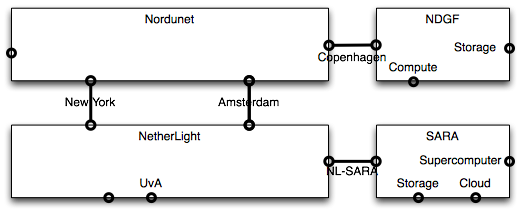
\includegraphics[width=390pt, height=159pt]{NSITopologyService-fig001.png}
\caption{Abstract view of an example NSI Topology}\label{fig:ndgf}
\end{center}
\end{figure}


\subsection{Introduction to concept of STPs}

 The basic network topology for the Network Service Interface (NSI) 
consists of networks, points and connections. The NSI can be used to request a 
connection between two different points, which is then implemented using the connection(s) 
between those points. Since each of the points in the network topology can terminate 
a network service, they are called Service Termination Points (STPs). The figure 
above contains several of these, for example the Storage point at SARA, another 
example is the connection point between the network on the edge of the SARA network 
which connects to the Netherlight network.\label{h.htn600ljqx1v}


\subsection{Identifying STPs in a request}

 The STPs in the Network Topology generally have two different 
roles:

 Endpoints within the network –points which are of interest to 
users, used as source and destination points

 One Part of a Service Demarcation Point (SDP) –meaning connections 
to other networks, used as transit points


 For the NSI network service, knowledge of the connections between 
networks is necessary to enable pathfinding. It is not strictly necessary to know 
all of the user endpoints in a network, as long as it is known in which network 
the endpoint is. It is assumed that once the network is reached, the endpoint within 
the network can be reached as well.

 To allow for pathfinding it is necessary that the Topology Service 
can identify the Networks, and the connections between those Networks, the SDPs. 
It is not necessary to distribute all of the endpoints within the network, which 
makes the distribution process much simpler.

 This means that a request to NSI must contain the source and destination 
network, as well as the connection points within those respective networks.


\subsection{Explicit routing using STPs}

 In a regular request only the source and destination STPs and 
their networks are specified. The selected path between those STPs is left to the 
NSA managing the request. In NSI v2.0 it is also possible to steer the requested 
path into a specific direction by defining intermediate STPs that the path must 
touch.

 Instead of a normal request with just a source and destination 
STP, the explicitly routed request will contain a path element which contains an 
indication of the path that should be taken through the NSI Network.

 If the Path object contains a description of the complete path 
end-to-end then this is simply a question of availability. However, problems can 
arise if the path object only contains a single ``explicit route object''(ERO) 
that it must touch. With the current NSI implementation and its bi-directional 
model, there is no way to know from which way to cross that ERO. The proposal is 
to use uni-directional path elements, to avoid ambiguity in the path direction 
(the uni-directionality of the ERO implicitly defines the direction).\label{h.4s5qtlwb3csi}


\subsection{Requirements for Topology Descriptions}

 Taking the description above into account, and with the general 
idea of the Network Service Interface in mind, we come to the following requirements 
for the network topology description:

 \textbf{Scalable} : An NSA does not need to be 
aware of all STPs in other networks;

 \textbf{Compact} : A Topology description should 
be able to group individual data transport capabilities in one object rather than 
specifying each possible VLAN for example;

 \textbf{Abstract} : The topology description 
should list the connections between domains, not how these connections are implemented;

 \textbf{Compatible} : It should be possible to 
relate the NSI topology to other topologies, e.g. as used for monitoring. Preferably 
the NSI topology should be compatible with the NML topology;

 \textbf{Flexible} : The topology description 
should support future extensions, e.g. different connection types (unidirectional, 
bidirectional, or multipoint connections), different levels of abstraction of the 
network (subtopologies), or multihoming scenarios;

 \textbf{Unambiguous} : The direction of an STP 
in an ERO should be unambiguous.\label{h.72kynww9xxpz}


\subsection{Proposal}

 To satisfy the unambiguity and flexibility requirements, we propose 
to describe STPs as two unidirectional Ports, since these have a single direction, 
there can be no misunderstanding. These unidirectional ports also easily allow 
point-to-multipoint requests.

 To satisfy the compact requirement, we propose to allow PortGroups 
over Ports. A PortGroup groups together several Ports which have a single identifying 
attribute, for example a VLAN label.

 To satisfy the scalability and flexibility requirement we propose 
to add the Topology ID as an added context for an STP in a request. This makes 
most of the global path through the network clear, without having specific knowledge 
about the internal endpoints. These can be handled by the NSAs responsible for 
those Topologies.

 To satisfy the compatibility and flexibility requirements we propose 
to use full URIs for each component in a request. Globally unique identifiers make 
it possible to have delegated subtopologies without having to rewrite identifiers 
for example.


 This means that a connection request for NSI should use the following 
tuple as source and destination:

 \textbf{(Topology ID, source PortGroup ID, sink PortGroup ID)}


\section{Topology Description Syntax}


\subsection{STP Identifiers}

 A source or destination of a connection reqest is identified by 
the Topology identifier and two unidirectional Ports or PortGroups. Each of these 
must be globally unique identifiers.

 A recommended way of constructing such an identifier is by using 
the \path{urn:ogf:network} namespace, for example \path{urn:ogf:network:example.net:2012:A1}.

 This identifer has three components: the prefix, urn:ogf:network 
which describes that it is a network identifier, the authoring namespace, example.net:2012 
which is the DNS name and a (at least) year to make a globally unique prefix\footnote{  
The date component in the identifier is optional but recommended. The DNS name 
is a temporary lease, which can change hands, so in order to guarantee uniqueness, 
the year component can be added.}, and the local component, A1 defined by the originating 
network. \label{h.nk6ov0u4wctm}


\subsection{STP Groups}

 Endpoints in a network often have a technology label associated 
with them, for example VLANs or wavelenghts. Rather than describing each of these 
available labels as individual STPs, we introduce the STP Group, equivalent to 
an NML PortGroup.

 An STP with a specific label can then be selected using the query 
component syntax as specified in [RFC3986], so for example:

\path{urn:ogf:network:example.net:2012:A2?vlan=1781} is a way to phrase 
a request to an STP with VLAN 1781 part of the STP Group identified by \path{urn:ogf:network:example.net:2012:A2}.


 If no specific label or attribute is given to select an STP from 
an STP group, the NSA for that network will select one from that STP group. The 
confirmation back to the requester will contain the fully specified STP selected 
for the request. An example for this kind of request is by specifying an STP which 
has VLAN labels, but not requesting a specific VLAN label. Continuing the example 
above, the STP \path{urn:ogf:network:example.net:2012:A2} has been specified to have a 
specific VLAN range available. A request with just that identifier as the destination 
will allow the pathfinder to select a VLAN on that specific endpoint, and return 
it to the user, using the query component.\label{h.p5scbjtwxk7s}


\subsection{DTOX Syntax}

 Version 1 of the NSI Connection Service specification left the 
topology definition out of scope. This has left a huge gap on the operational side, 
where implementers have had to cooperate to create a common file to represent the 
topologies of each of the domains, and how to share that data. The Distributed 
TOpology eXchange (DTOX) working group of GLIF jumped to the opportunity and quickly 
provided a topology format. This was heavily inspired by the NML work in progress, 
but also contained some additions specific to NSI. This has allowed us to gain 
some experience in required elements for a topology format, and the way it could 
be exchanged.\


 The current DTOX format contains the following elements:

 \begin{description}

   \item[\textbf{STP}] Service Termination Point.

   \item[\textbf{connectedTo}]  relation to form an SDP 
  with another STP

   \item[\textbf{NSNetwork}]  Network Service Network

   \item[\textbf{hasSTP }] to define STP containment

   \item[\textbf{locatedAt}]  to define a location of a network
   \item[\textbf{Location}]

   \item[\textbf{lat, long}]  define GPS coordinates

   \item[\textbf{NSA}]  Network Service Agent

   \item[\textbf{managing}  to relate it to an  \textbf{NSNetwork}]

   \item[\textbf{adminContact}]  to describe contacts for the administrator

   \item[\textbf{csProviderEndpoint}]  to define the URL at which the NSA is reachable

 \end{description}


 The above format is simple, but has proven to be very effective. 
The STP elements are the most important ones which provide the identifiers and 
connectivity information necessary to do path calculations between domains.

 The NSI topology representation will make use the NML topology 
representation as much as possible to build on standardized work in that group. 
This will be extended with some NSI specific terminology as shown in Figure~\ref{fig:ndgf}.

\begin{table}
  \begin{center}

  \begin{tabular}{|l|l|}
\hline
% ROW 1
\textit{NSI Concept} & \textit{Representation}\\
\hline
% ROW 2
STP & 2x 
\texttt{nml:Port} / \texttt{nml:BidirectionalPort}\\
\hline
% ROW 3
Connected To & \texttt{nml:alias}\\
\hline
% ROW 4
NSNetwork & \texttt{nml:Topology}\\
\hline
% ROW 5
Has STP & \texttt{nml:hasPort}\\
\hline
% ROW 6
Located at & \texttt{nml:locatedAt}\\
\hline
% ROW 7
Location & \texttt{nml:Location}\\
\hline
% ROW 8
GPS coords & \texttt{nml:lat}, 
\texttt{nml:long}\\
\hline
% ROW 9
NSA & \texttt{nsi:NSA}\\
\hline
% ROW 10
Network managed by NSA & \texttt{nsi:managedBy}\\
\hline
% ROW 11
Admin Contact & \texttt{nsi:adminContact}\\
\hline
% ROW 12
Provider endpoint URL & \texttt{nsi:csProviderEndpoint}\\
\hline
% ROW 13
Control-plane connections & \texttt{nsi:peersWith}\\
\hline
\end{tabular}
\caption{Relation of NSI and NML terminology}\label{tab:nsi-nml}
  \end{center}
\end{table}


\subsection{Topology Description Example}

 A simple example NSI Network topology description is provided 
below. This example describes only the NDGF network as depicted in Figure~\ref{fig:ndgf}. The 
complete topology description for Figure~\ref{fig:ndgf} is available in Appendix~\ref{app:A}.

\begin{verbatim}
  ndgf:NordicDataGridFacility a nml:Topology ;
          nml:version "2011112901" ;
          nml:name "NDGF" ;
          nml:locatedAt ndgf:location ;
          nml:hasOutboundPort ndgf:dk-ndgf-nordunet ;
          nml:hasInboundPort ndgf:nordunet-dk-ndgf ;
          nml:hasOutboundPort ndgf:ndgf-storage ;
          nml:hasInboundPort ndgf:storage-ndgf ;
          nsi:managedBy ndgf:nsa .
  ndgf:location a nml:Location ;
          nml:lat "55.637"^^<http://www.w3.org/2001/XMLSchema#float> ;
          nml:long "12.641"^^<http://www.w3.org/2001/XMLSchema#float> .
  ndgf:nsa a nsi:NSA ;
          nsi:csProviderEndpoint "http://nsa.ndgf.org/" .
  ndgf:dk-ndgf-nordunet a nml:PortGroup ;
          nmleth:vlans "1780-1783" ;
          nml:alias nordunet:dk-ndgf-nordunet .
  ndgf:nordunet-dk-ndgf a nml:PortGroup ;
          nmleth:vlans "1780-1783" ;
          nml:alias nordunet:nordunet-dk-ndgf .
  ndgf:ndgf-storage a nml:PortGroup ;
          nmleth:vlans "1780-1783" .
  ndgf:storage-ndgf a nml:PortGroup ;
          nmleth:vlans "1780-1783" .
\end{verbatim}



 The above example provides the minimal information to expose, 
a Topology, a Location, an NSA, two PortGroups for the connection with NorduNet, 
and finally two PortGroups describing the Storage endpoint in the network, all 
with VLAN ranges.

 The Topology element is used to hide internal connectivity, and 
a full-mesh is assumed. By adding more NML topology information, it is possible 
to include more detailed descriptions of the internal network.


 The NSA provides the management information for networks, how 
the NSI interface can be reached, and who actually maintain the NSA.

 The Location element has also proven to be quite useful in allowing 
us to quickly create stunning visualizations using Google Earth.\label{h.xynx25fm6som}


\subsection{Subtopologies}

 A topology can be further subdivided into subtopologies if required. 
If for example NORDUnet decides to split their USA and Scandinavian networks, we 
end up with a topology such as shown in figure~\ref{fig:ndgf2}.

\begin{figure}[htbp]
\begin{center}
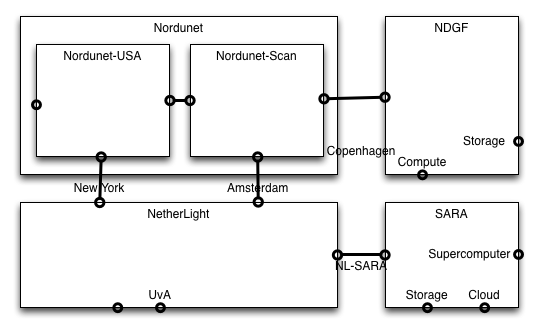
\includegraphics[width=403pt, height=248pt]{NSITopologyService-fig002.png}
\caption{An example topology where Nordunet uses subtopologies}\label{fig:ndgf2}
\end{center}
\end{figure}


 If described correctly, the other domains do not have to update 
their topologies or connections. NORDUnet just updates its version number, and 
makes a new topology file available with subtopologies. The description of the 
new NORDUnet topology is given at the end of Appendix A.\label{h.ikfi9yd4mu6x}


\section{Distribution of NSI Topology}

 Some form of Topology distribution is required in order for an 
inter-domain NSI network to function. In NSI 1.0 this process was performed out-of-band, 
mostly through e-mail. For NSI 2.0 we take the opportunity to define an NSI Topology 
Service for NSI topology exchange, which can support the NSI Connection Service.\label{h.c2129mkn366h}


\subsection{Transport and Service plane relationship}

 The NSI Connection Service is implemented on Network Service Agents 
(NSAs), which together form a network and tree-like structure. This graph represents 
how reservation requests would propagate through the network, but not necessarily 
reflects the transport-plane. One NSA may be an aggregation point for other NSAs, 
not visible from the outside.\label{h.mtia1ajwgzmv}


The messaging between the NSAs will happen on the 
service plane, which is completely separate from the transport plane.\label{h.dc66uw3zo12t}\label{h.ywjdj9kuwkou}


\subsection{Elements of a Topology Exchange Mechanism}

 There are three main elements of topology exchange: \label{h.u0b214m8krs}


\paragraph{Bootstrapping Topology Exchange}

 To start the initial Network Service the NSAs must be able to 
find each other, in order to communicate details about the network. So some form 
of bootstrapping is required, with initial synchronization between domains on both 
the service plane and the transport plane, i.e. the NSAs of both domains must be 
able to contact each other, and the details of transport plane connections between 
them have to be synchronized as well.\label{h.fzohc79rts8y}


Initiating a transport plane connection between two 
networks is not a frequent occurrence, and a longer process, involving out-of-band 
(for NSI) contact. Part of that process can be that the networks also communicate 
the access details for the NSAs, thus forming an NSA relationship.\label{h.30v92h80y7jj}


\paragraph{Expanding the Topology Exchange}

 Once the neighboring (on the control-plane) NSAs have exchanged 
details, they can also distribute details about the rest of the network, both the 
control plane details and connectivity, but also some transport details.\label{h.c1dz1g10oju}

\paragraph{Update Mechanism}

 The transport network is not static, and links are added or removed 
from time to time. An update mechanism is thus required to inform other NSAs about 
these kinds of events.\label{h.uzmy62lgeii3}


\subsection{Topology Exchange Implementations}

 The above mechanisms can be implemented in five different ways:


\paragraph{Centralized Manual Distribution}
 An initial attempt at topology distribution in the Automated GOLE 
demonstration was through a central maintainer. This maintainer collected all topology 
information from the networks involved, gathered all the topology data and sent 
out a topology file through e-mail. The network maintainers would than download 
the attachment and insert it into their provisioning system. Updates to the topology 
were all handled through the central maintainer, distributed through e-mail.\label{h.31tbtceozcoc}


While this system worked initially, it soon ran into 
scaling problems. This system also does not allow to have a good way of doing automatic 
updates or insertion.


\paragraph{Version Controlled Distribution}

 The Automated GOLE demonstration has transitioned into a different 
distribution mechanism using a Git source code repository, available on GitHub. 
This mechanism also still has a central maintainer, this also allows networks to 
manipulate their own topology information. The distribution mechanism is either 
directly from the GitHub website, or through the git version control system itself. 
The git system has the added advantage that it is a distributed version control 
system, so it is not required to download directly from GitHub.\label{h.rtljwvhj8cbo}


Bootstrapping and updating all happens through the 
git system itself.


\paragraph{PerfSonar Lookup Service}

 The PerfSonar monitoring system suite also contains a service 
for looking up information. This service uses a ``home Lookup Service''(hLS) where 
metadata of information is registered, which is then uploaded into the ``global 
Lookup Service''(gLS) (this can be cloud of services).\label{h.pg14lxc0zu6o}


The retrieval of information happens by first querying 
the gLS, then the relevant hLS, followed by the service where the actual information 
is stored.\label{h.tjjrmby8htjk}


Since topology information would be stored locally, 
no update mechanism is necessary, except for location changes of the services itself. 
However, this method of storing and lookup does require full connectivity between 
all NSAs to provide and retrieve information, which may not be possible.


 A soon to be released (target Dec 2012) updated PS Lookup service 
will incorporate subscription capabilities, which allow an hLS to push information 
to a remote hLS and have it cached locally there. By adapting the new Lookup service 
to store topology, and selectively managing the subscription of data, full connectivity 
between NSAs would not be necessary to disseminate global topology.


\paragraph{HTTP Distribution}

 A common way of distributing information is using the HTTP protocol. 
The topology files would include links to topology description files, which would 
allow other domains to directly fetch the topology description.\label{h.efkcsmt7dwgr}


However, as with the Lookup Service, this requires 
direct access between NSAs which may not be possible.\label{h.mbgns4xsvbt4}


\paragraph{A Peer-to-Peer Distribution Protocol}

 Another method is to define a new protocol for NSI topology distribution. 
As explained above the protocol would only require a small set of primitives, and 
would work directly between peering NSAs.\label{h.jo1it2zr3py}


Once an NSA comes up, it contacts its neighbors to 
request the topology information that they know about, and subscribes to future 
topology updates. These updates are propogated in a peer-to-peer fashion through 
the whole network.\label{h.3qkmh8hazvti}


The end-result would be that all the NSAs have a 
global view of the topology, with only local interaction.\label{h.40nvr2if8zj}


\subsection{Summarizing Topology Distribution}

 Above we have described five different topology distribution mechanisms, 
from these five only the version controlled and peer-to-peer systems fit the requirements 
that the NSI has, others require too much manual operation, or require globally 
reachable NSAs. The peer-to-peer system would be the best solution with minimal 
interaction between systems, and no reliance on outside mechanisms. For practical 
reasons we believe the best solution right now is a version controlled distribution 
system, and in time evolve to a peer-to-peer distribution protocol.\label{h.j5x37xsutbrh}


\section*{Appendix A –Example Topology Description}\label{app:A}

 Below is the complete topology description of Figure~\ref{fig:ndgf} written 
in NML using the Notation3 syntax.

\begin{verbatim}
  @prefix nml:        <http://schemas.ogf.org/nml/2012/10/base#> .
  @prefix nmleth:     <http://schemas.ogf.org/nml/ethernet/2012/10#> .
  @prefix nsi:        <http://schemas.ogf.org/nsi/topology/2012/10#> .
  @prefix ndgf:       <urn:ogf:network:ndgf.org:2012:> .
  @prefix nordunet:   <urn:ogf:network:nordu.net:2012:> .
  @prefix nl:         <urn:ogf:network:netherlight.net:2010:> .
  @prefix sara:       <urn:ogf:network:sara.nl:2011:> .

  ndgf:NordicDataGridFacility a nml:Topology ;
          nml:version "2011112901" ;
          nml:name "NDGF" ;
          nml:locatedAt ndgf:location ;
          nml:hasOutboundPort ndgf:dk-ndgf-nordunet ;
          nml:hasInboundPort ndgf:nordunet-dk-ndgf ;
          nml:hasOutboundPort ndgf:ndgf-storage ;
          nml:hasInboundPort ndgf:storage-ndgf ;
          nsi:managedBy ndgf:nsa .
  ndgf:location a nml:Location ;
          nml:lat "55.637"^^<http://www.w3.org/2001/XMLSchema#float> ;
          nml:long "12.641"^^<http://www.w3.org/2001/XMLSchema#float> .
  ndgf:nsa a nsi:NSA ;
          nsi:csProviderEndpoint "http://nsa.ndgf.org/" .
  ndgf:dk-ndgf-nordunet a nml:PortGroup ;
          nmleth:vlans "1780-1783" ;
          nml:alias nordunet:dk-ndgf-nordunet .
  ndgf:nordunet-dk-ndgf a nml:PortGroup ;
          nmleth:vlans "1780-1783" ;
          nml:alias nordunet:nordunet-dk-ndgf .
  ndgf:ndgf-storage a nml:PortGroup ;
          nmleth:vlans "1780-1783" .
  ndgf:storage-ndgf a nml:PortGroup ;
          nmleth:vlans "1780-1783" .

  nordunet:Nordunet a nml:Topology ;
          nml:version "2012061801" ;
          nml:name "Nordunet" ;
          nml:hasOutboundPort nordunet:nordunet-dk-ndgf ;
          nml:hasOutboundPort nordunet:nordunet-surfnet-NYC ;
          nml:hasOutboundPort nordunet:nordunet-surfnet-AMS ;
          nml:hasInboundPort nordunet:dk-ndgf-nordunet ;
          nml:hasInboundPort nordunet:surfnet-NYC-nordunet ;
          nml:hasInboundPort nordunet:surfnet-AMS-nordunet .
  nordunet:nordunet-dk-ndgf a nml:PortGroup ;
          nmleth:vlans "1780-1783" ;
          nml:alias ndgf:nordunet-dk-ndgf .
  nordunet:dk-ndgf-nordunet a nml:PortGroup ;
          nmleth:vlans "1780-1783" ;
          nml:alias ndgf:dk-ndgf-nordunet .
  nordunet:nordunet-surfnet-AMS a nml:PortGroup ;
          nmleth:vlans "1780-1783" ;
          nml:alias nl:nordunet-surfnet-AMS .
  nordunet:nordunet-surfnet-NYC a nml:PortGroup ;
          nmleth:vlans "1780-1783" ;
          nml:alias nl:nordunet-surfnet-NYC .
  nordunet:surfnet-AMS-nordunet a nml:PortGroup ;
          nmleth:vlans "1780-1783" ;
          nml:alias nl:surfnet-AMS-nordunet .
  nordunet:surfnet-NYC-nordunet a nml:PortGroup ;
          nmleth:vlans "1780-1783" ;
          nml:alias nl:surfnet-NYC-nordunet .

  nl:NetherLight a nml:Topology ;
          nml:version "2011062101" ;
          nml:name "NetherLight" ;
          nml:hasOutboundPort nl:surfnet-NYC-nordunet ;
          nml:hasOutboundPort nl:surfnet-AMS-nordunet ;
          nml:hasOutboundPort nl:surfnet-SARA ;
          nml:hasInboundPort nl:nordunet-surfnet-NYC ;
          nml:hasInboundPort nl:nordunet-surfnet-AMS ;
          nml:hasInboundPort nl:SARA-surfnet .
  nl:nordunet-surfnet-AMS a nml:PortGroup ;
          nmleth:vlans "1780-1783" ;
          nml:alias nordunet:nordunet-surfnet-AMS .
  nl:nordunet-surfnet-NYC a nml:PortGroup ;
          nmleth:vlans "1780-1783" ;
          nml:alias nordunet:nordunet-surfnet-NYC .
  nl:SARA-surfnet a nml:PortGroup ;
          nmleth:vlans "1780-1783" ;
          nml:alias sara:SARA-surfnet .
  nl:surfnet-AMS-nordunet a nml:PortGroup ;
          nmleth:vlans "1780-1783" ;
          nml:alias nordunet:surfnet-AMS-nordunet .
  nl:surfnet-NYC-nordunet a nml:PortGroup ;
          nmleth:vlans "1780-1783" ;
          nml:alias nordunet:surfnet-NYC-nordunet .
  nl:surfnet-SARA a nml:PortGroup ;
          nmleth:vlans "1780-1783" ;
          nml:alias sara:surfnet-SARA .


  sara:SARA a nml:Topology ;
          nml:version "2010072401" ;
          nml:name "SARA" ;
          nml:hasOutboundPort sara:SARA-surfnet ;
          nml:hasInboundPort sara:surfnet-SARA .
  sara:SARA-surfnet a nml:PortGroup ;
          nmleth:vlans "1780-1783" ;
          nml:alias nl:SARA-surfnet .
  sara:surfnet-SARA a nml:PortGroup ;
          nmleth:vlans "1780-1783" ;
          nml:alias nl:surfnet-SARA .
\end{verbatim}



 An example of an updated topology for NorduNet with subtopologies. 
This new topology does not require any changes on the other network topologies.

\begin{verbatim}
nordunet:Nordunet a nml:Topology ;
        nml:version "2012080401" ;
        nml:name "Nordunet" ;
        nml:hasTopology nordunet:NordunetScandinavia ;
        nml:hasTopology nordunet:NordunetUSA .

nordunet:NordunetScandinavia a nml:Topology ;
        nml:version "2012080401" ;
        nml:name "Nordunet Scandinavia" ;
        nml:hasOutboundPort nordunet:nordunet-dk-ndgf ;
        nml:hasOutboundPort nordunet:nordunet-surfnet-AMS ;
        nml:hasOutboundPort nordunet:Scan-to-USA-trunk ;
        nml:hasInboundPort nordunet:dk-ndgf-nordunet ;
        nml:hasInboundPort nordunet:surfnet-AMS-nordunet ;
        nml:hasInboundPort nordunet:Scan-from-USA-trunk .
nordunet:dk-ndgf-nordunet a nml:PortGroup ;
        nml:alias ndgf:dk-ndgf-nordunet .
nordunet:nordunet-dk-ndgf a nml:PortGroup ;
        nml:alias ndgf:nordunet-dk-ndgf .
nordunet:nordunet-surfnet-AMS a nml:PortGroup ;
        nml:alias nl:nordunet-surfnet-AMS .
nordunet:Scan-from-USA-trunk a nml:PortGroup ;
        nml:alias nordunet:USA-to-Scan-trunk .
nordunet:Scan-to-USA-trunk a nml:PortGroup ;
        nml:alias nordunet:USA-from-Scan-trunk .
nordunet:surfnet-AMS-nordunet a nml:PortGroup ;
        nml:alias nl:surfnet-AMS-nordunet .

nordunet:NordunetUSA a nml:Topology ;
        nml:version "2012080401" ;
        nml:name "Nordunet USA" ;
        nml:hasOutboundPort nordunet:nordunet-surfnet-NYC ;
        nml:hasOutboundPort nordunet:USA-to-Scan-trunk ;
        nml:hasInboundPort nordunet:surfnet-NYC-nordunet ;
        nml:hasInboundPort nordunet:USA-from-Scan-trunk .
nordunet:nordunet-surfnet-NYC a nml:PortGroup ;
        nml:alias nl:nordunet-surfnet-NYC .
nordunet:surfnet-NYC-nordunet a nml:PortGroup ;
        nml:alias nl:surfnet-NYC-nordunet .
nordunet:USA-from-Scan-trunk a nml:PortGroup ;
        nml:alias nordunet:Scan-to-USA-trunk .
nordunet:USA-to-Scan-trunk a nml:PortGroup ;
        nml:alias nordunet:Scan-from-USA-trunk .
\end{verbatim}


\end{document}
